\chapter{Calibration Results \label{ch:calibration_results}}
The program \verb|att_eval.py| introduced in section~\ref{sec:meth:data_interpretation} is used to evaluate the calibration measurement and flight data. This chapter presents the results of the calibration measurement. From this measurement we choose a set of optimal coefficients for the accelerometer and magnetometer, as introduced in sec.~\ref{sec:meth:calibration_technique} on page~\pageref{sec:meth:calibration_technique}. We then analyse the flight data's attitude and heading information calibrated with these coefficients.

Figure~\ref{fig:res:raw_cali} presents the unfiltered measurements of the magnetometer. Only a 2D image of the 3D plot is shown to convey two important things: Firstly the axes are scaled to the same range to show that the measurements form an ellipsoid rather than a sphere. Secondly some spots can be seen, which do not lie on the ellipsis, as well as some single measurement points distributed throughout the figure. The first step in the calibration is to eliminate these statistical outliers. We eliminate them as they do not contribute to the calibration in a meaningful way because their existence is not systematic, intrinsic to the sensors, but is a chance occurrence. The surface of the ellipsoid is not smooth because like any measurement the measurement points, in this case magnetic field vectors, are distributed around the true value. 

\begin{figure}[H]
    \centering
    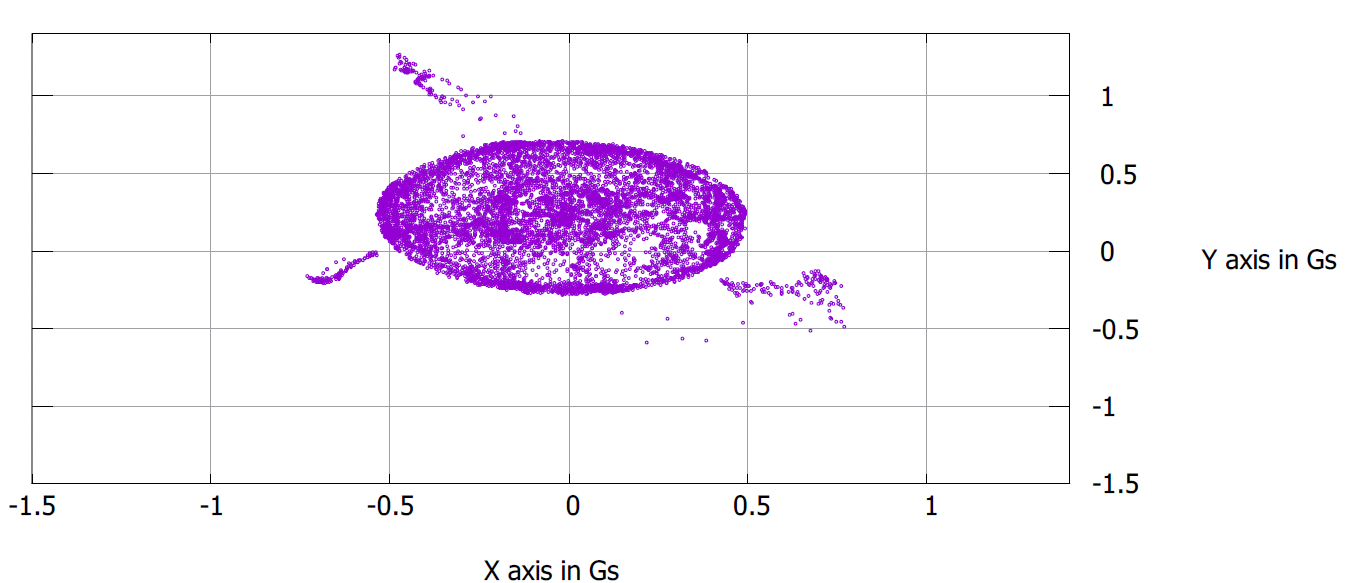
\includegraphics[width=\linewidth]{images/04_calibration/raw_sphere_2025-04-11_x_y_axes.png}
    \caption[Magnetometer components of the calibration measurement on 11 April 2025 plotted in 3D-Space to form a distorted sphere.]{Magnetometer components of the calibration measurement on 11 April 2025 plotted in 3D-Space to form a distorted sphere. The x- and y-axes are shown with the same axis scaling to illustrate the different offsets and scale factors of the axes.}
    \label{fig:res:raw_cali}
\end{figure}

A clear distinction between three time intervals can be made in fig.~\ref{fig:res:raw_cali_vectors}. The first interval is from the beginning of the measurement until 9:55. This is the time it took to leave the lab, take the elevator to the basement and go to the car park. Quite a lot of vibration can be seen in the accelerometer and stray magnetic fields measured by the magnetometer.\\
The second phase is from 9:55 to around 10:21, after when the random tumble begins. In phase II, it can be seen how the magnetometer and accelerometer react to laying the device housing down in different orientations. When rotating the sensors, small shocks can be seen, such as at 10:06. These shocks are a different type of outlier than described in the previous paragraph for fig.~\ref{fig:res:raw_cali}. They determine the thickness of the ellipsoid's mantle. The magnitude of the field randomly decreases significantly, leading to measurement points near the centre of the sphere.

\begin{figure}[H]
    \centering
    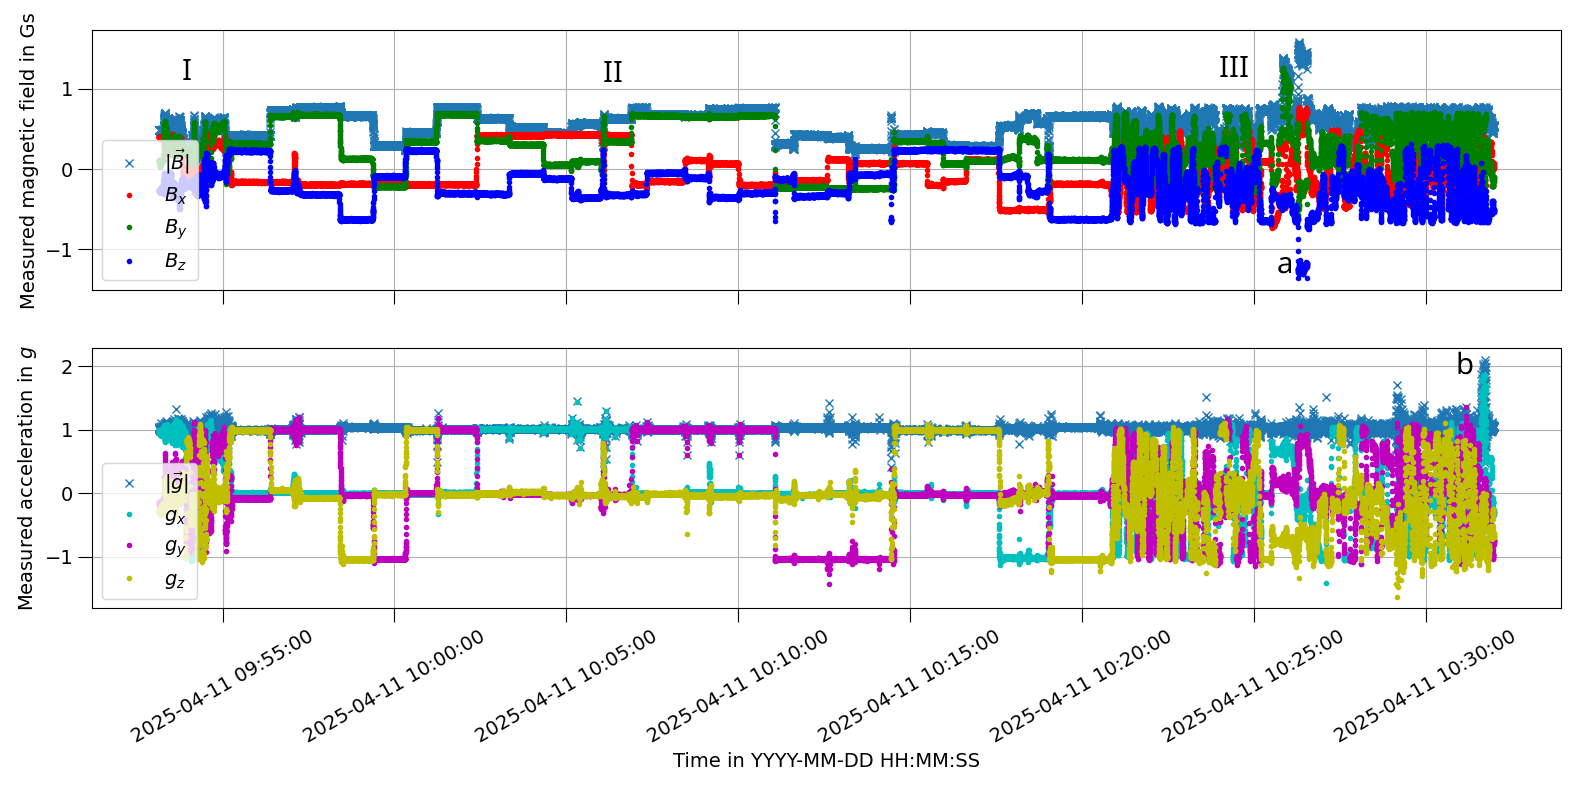
\includegraphics[width=\linewidth]{images/04_calibration/raw_vectors-2025-04-11.png}
    \caption[Components of the magnetometer and accelerometer plotted against time.]{Components of the magnetometer and accelerometer plotted against time. Shown with blue crosses is the sum of the squares of the components, i.e. the length of the measured vector. Noted in the upper image are the three phases I, II and III. Marked with a and b are two outliers cut from the dataset for the calibration.}
    \label{fig:res:raw_cali_vectors}
\end{figure}

There is one very important thing we can learn from figure~\ref{fig:res:raw_cali_vectors}. The three axes of the magnetometer have vastly different offsets and scale factors. The measured field's magnitude should be roughly constant throughout the whole time of phases II and III when the device is brought outside, away from any hard iron sources. However, looking at 10:00, it is obvious that this is not the case, showing that the offsets and scale factors are different for each axis and not yet determined. It is visible that no particularly sudden or strong accelerations are experienced during the random tumble. However, for some reason, the magnetometers measured field goes up to about $1.5\,\mathrm{Gs}$, which is around 6 times the field strength in Kiel (for reference, see sec.~\ref{sec:da:vector_fields}). This sudden spike in magnetic field strength can not be linked to any particular event observed during testing. \\
We perform three approximations of the calibration parameters. The first only takes phase II into account, the second only phase III, and a third approximation with both phases. In fig.~\ref{fig:res:raw_calibration_three_phases} the components of the magnetometer are shown in three dimensional space to illustrate the different behaviours during the measurement methods of placing the magnetometer in a single position for a longer duration of time (fig.~\ref{fig:res:raw_calibration_three_phase_II}) leading to a few large spots on the sphere, and the random tumble (fig.~\ref{fig:res:raw_calibration_three_phase_III}) resulting in a sphere with a homogenous surface density of spots. The time intervals around 10:26 and 10:32 (a and b in the image) where magnetometer and accelerometer magnitude are significantly higher have been cut as well as phase I. This improves the accuracy of the final parameters. This also eliminates all the outliers discussed in fig.~\ref{fig:res:raw_cali}, as can be seen by comparing to fig.~\ref{fig:res:raw_calibration_three_phases}.

\begin{figure}[h]
\begin{subfigure}[t]{.33\textwidth}
  \centering
  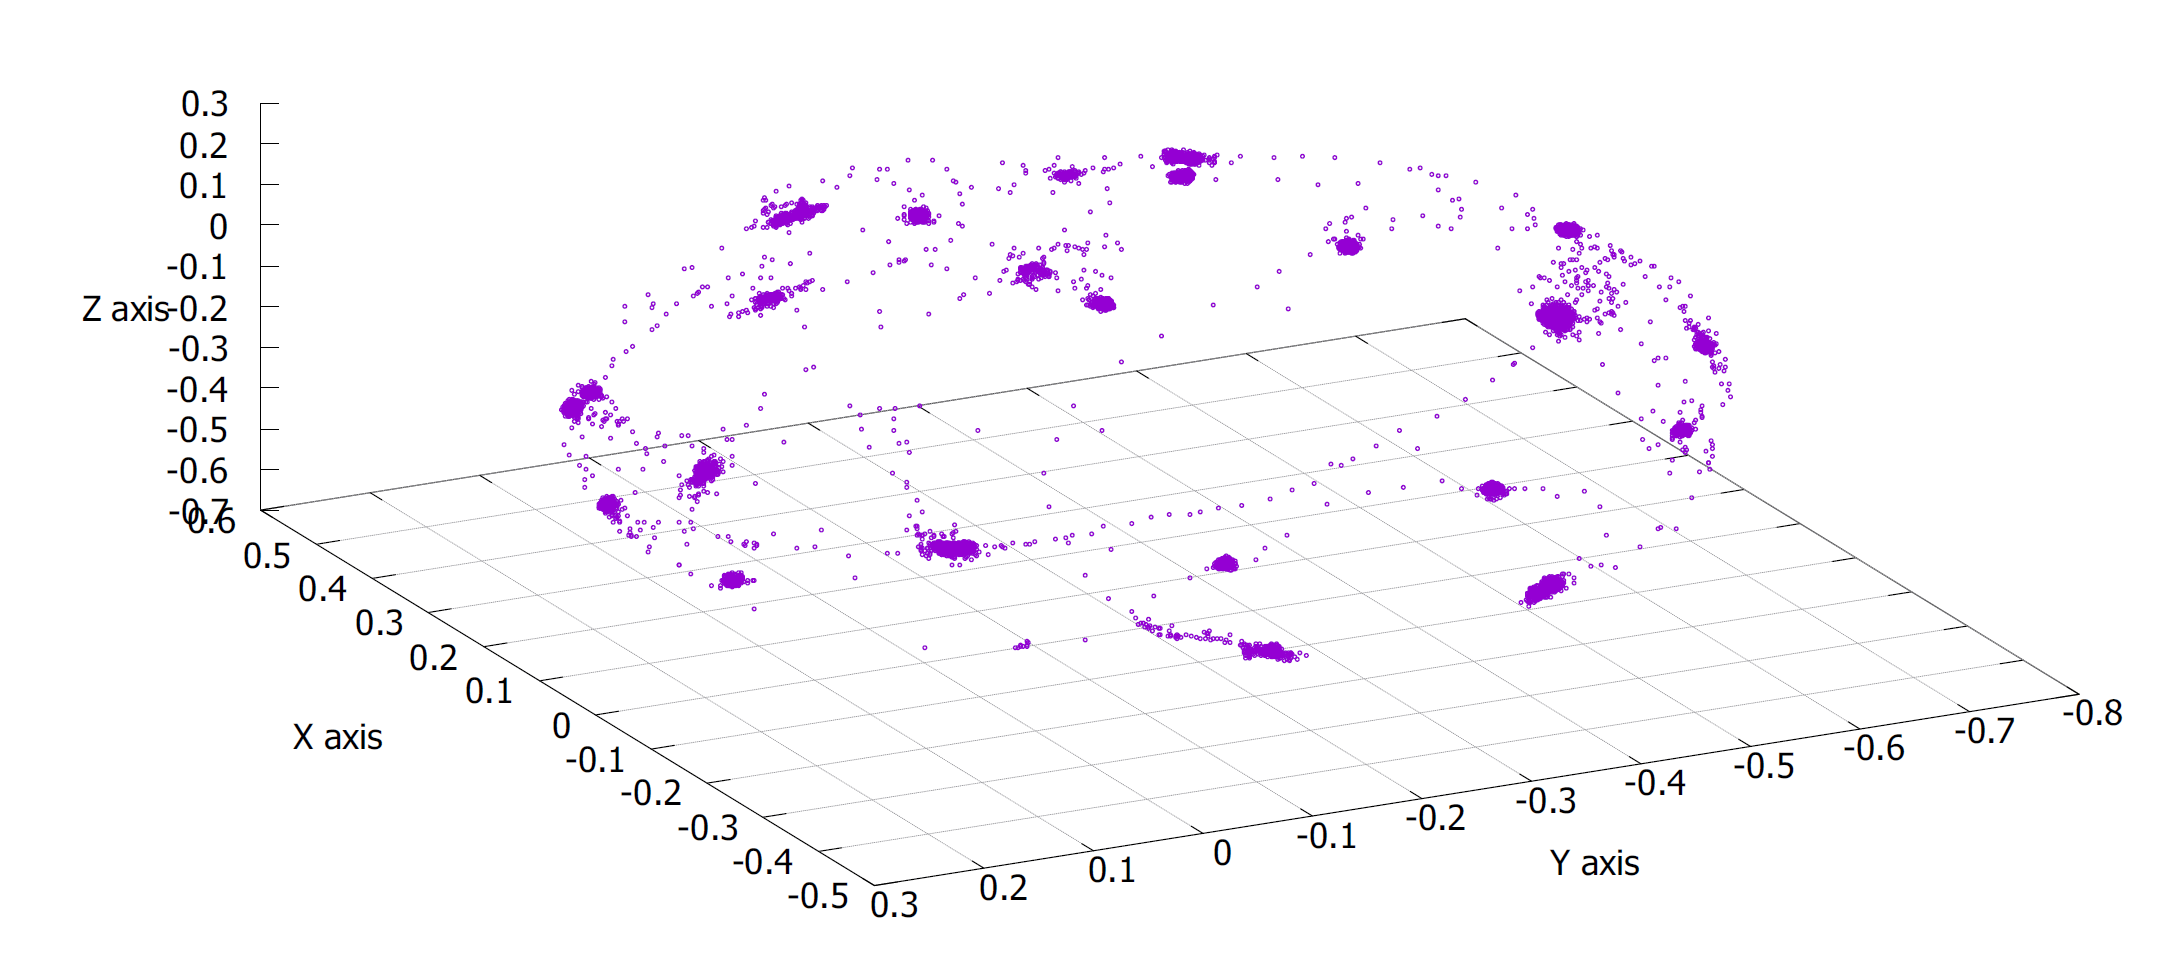
\includegraphics[width=.8\linewidth]{images/04_calibration/raw_sphere_calibration_phase_II.png}
  \caption{Phase II, multiple orientations.}
  \label{fig:res:raw_calibration_three_phase_II}
\end{subfigure}%
\begin{subfigure}[t]{.33\textwidth}
  \centering
  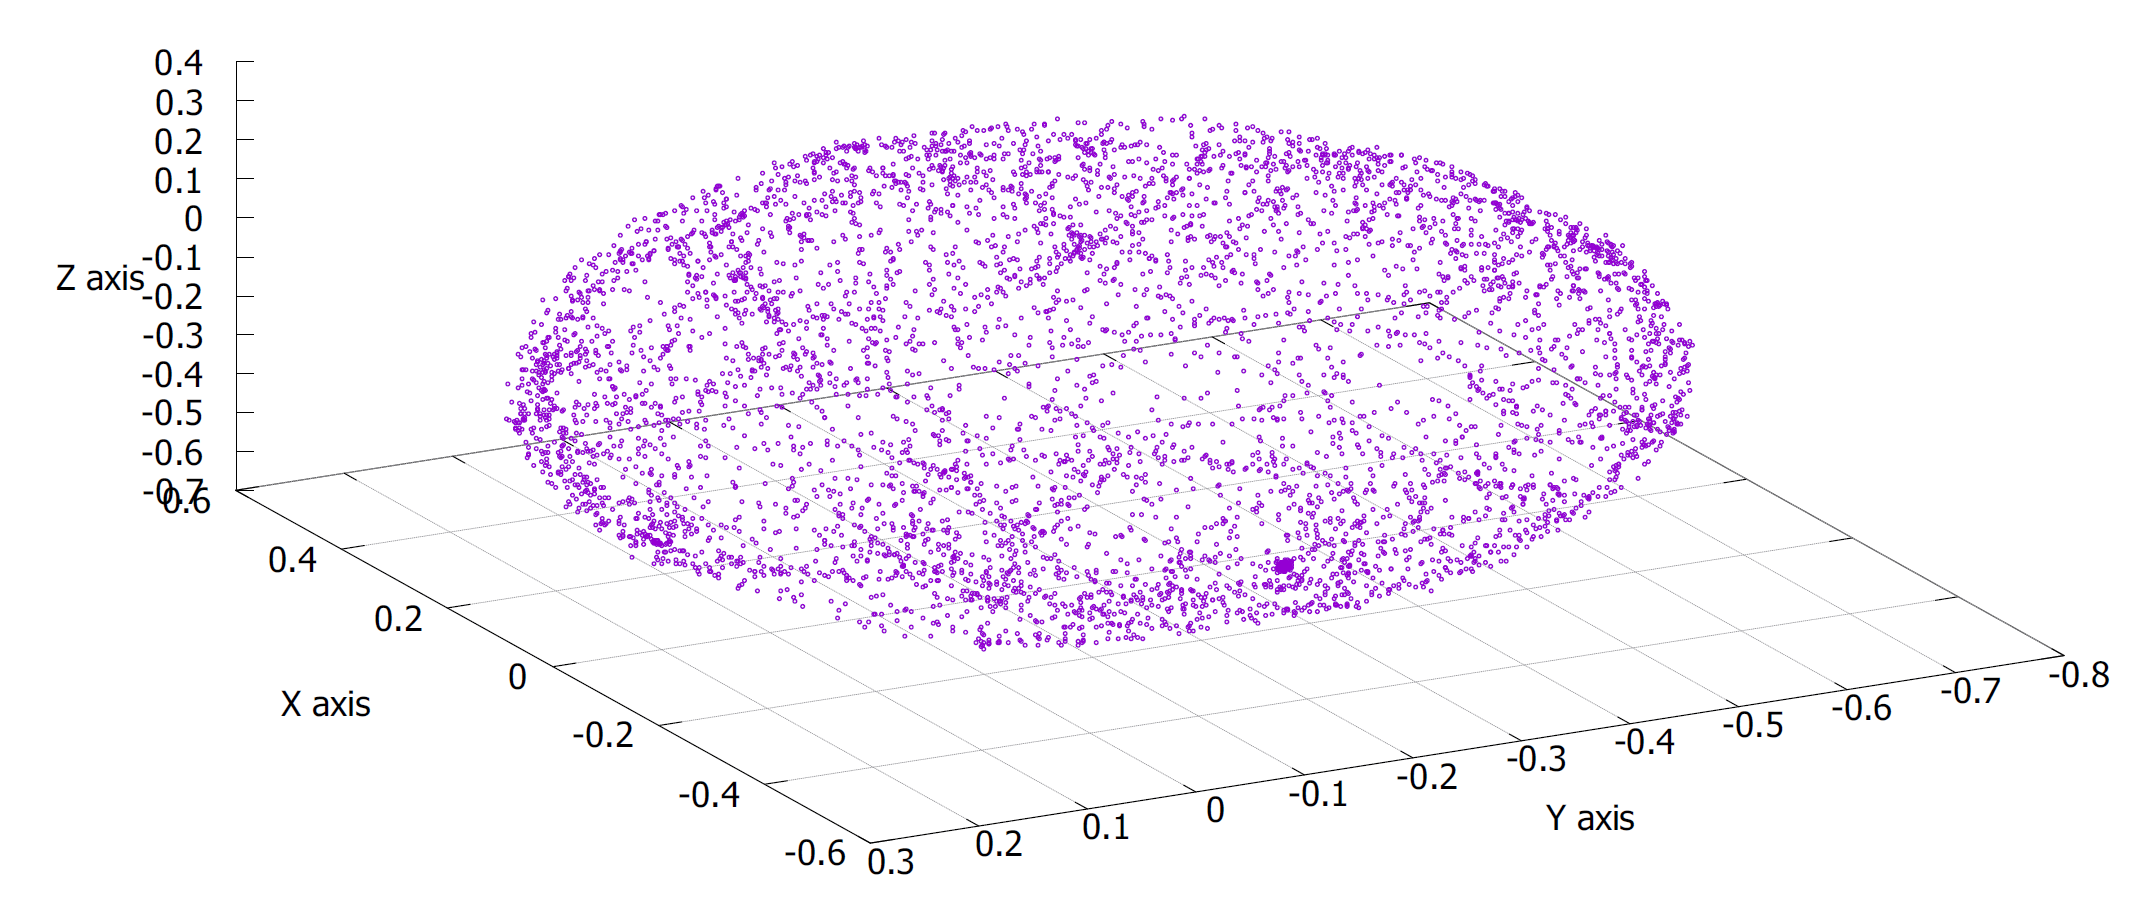
\includegraphics[width=.8\linewidth]{images/04_calibration/raw_sphere_calibration_phase_III.png}
  \caption{Phase III, random tumble.}
  \label{fig:res:raw_calibration_three_phase_III}
\end{subfigure}
\begin{subfigure}[t]{.33\textwidth}
  \centering
  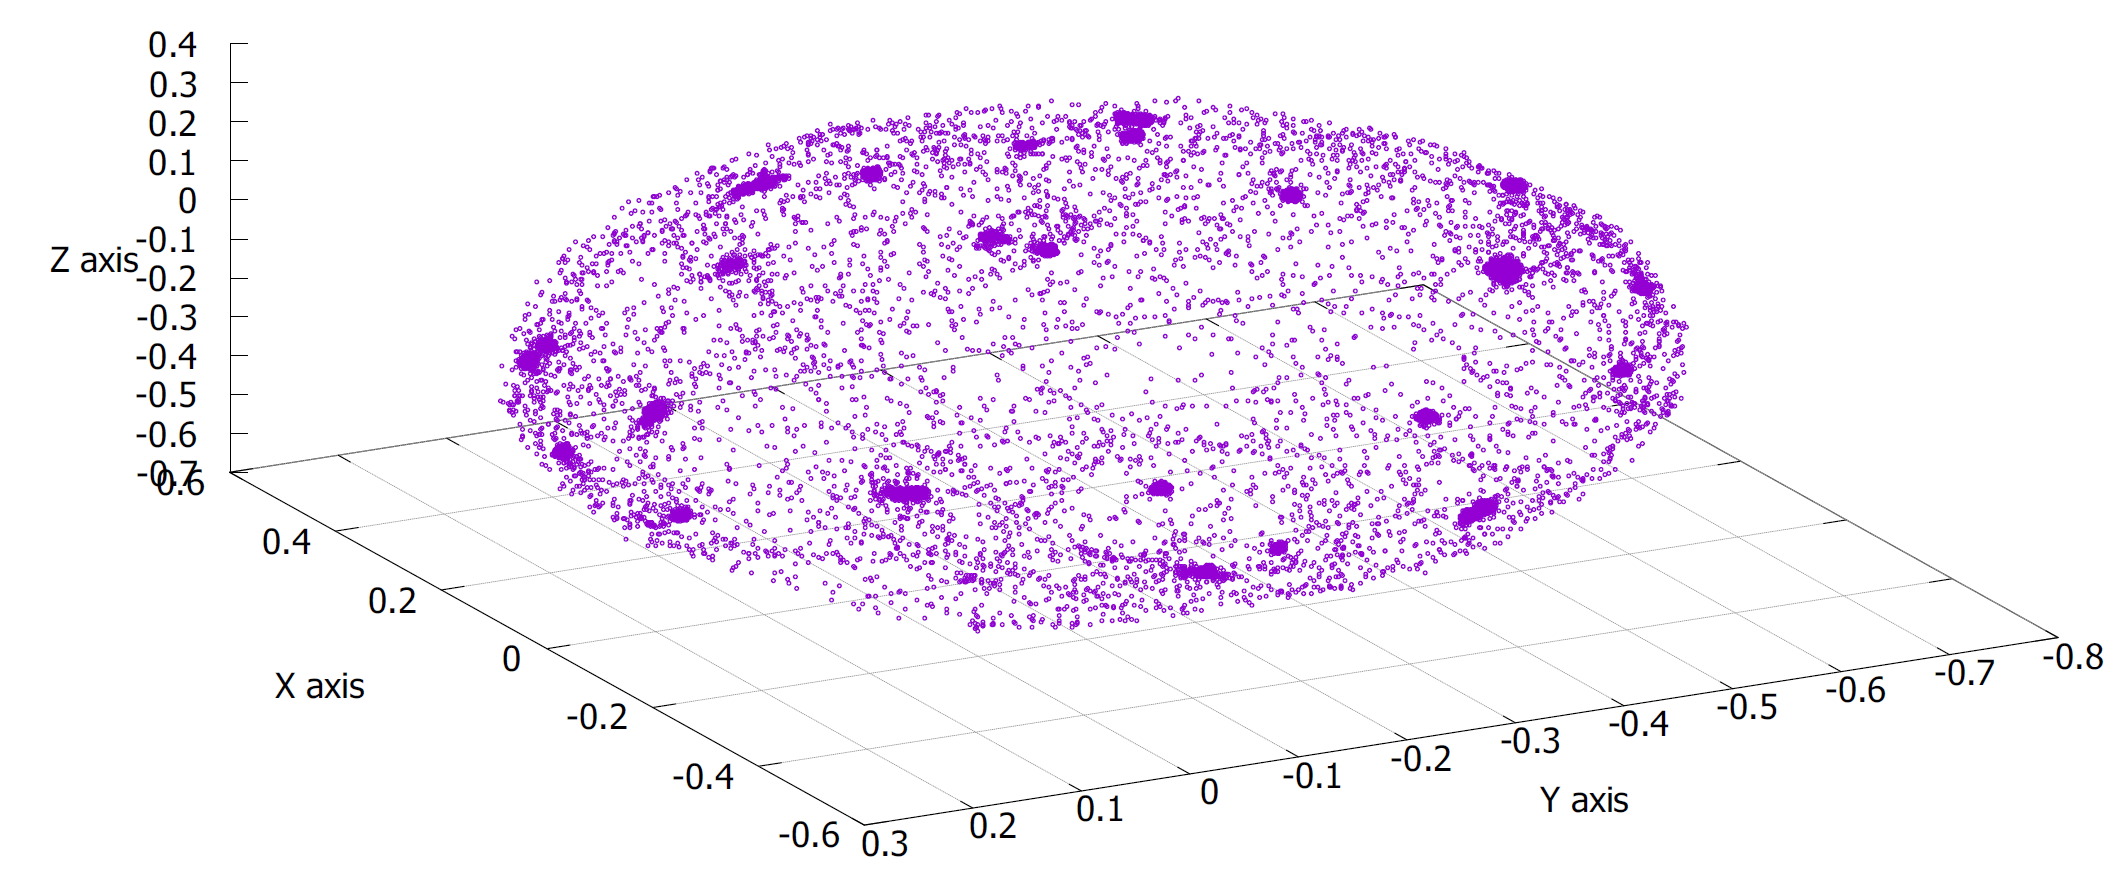
\includegraphics[width=.8\linewidth]{images/04_calibration/raw_sphere_calibration_phases_II_III.png}
  \caption{Phases II and III, combination of both.}
\end{subfigure}
\caption{Uncalibrated magnetometer components of the calibration measurement plotted in 3D-Space to form a distorted sphere.}
\label{fig:res:raw_calibration_three_phases}
\end{figure}


Section~\ref{sec:app:final_coefficients} presents the final fit parameters in table~\ref{tab:app:coeff}, and the correlation matrices later in the same section. The measurements are calibrated using all three sets and the residuals, i.e. the difference between the calibrated vector and the theoretical value, are calculated to determine the best set of parameters. 

Figure~\ref{fig:res:residuals} presents the residuals (for a further explanation, see page~\pageref{eq:residuals}) with mean $\mu$ and standard deviation $\sigma$. It can be seen that the magnetometer calibration with the lowest mean deviation from the optimal value of $503.4\,\mathrm{mGs}$ is the calibration using phases~II~+~III. The accelerometer calibration with the lowest deviation from the optimal value of 1$g$ uses only phase~II. This can be explained with the unwanted accelerations when moving the sensor in a circular motion.\\
All sets of coefficients have approximately the same standard deviations, which are about 50 to 100 times larger than the means. This can be explained by the extremely large errors in the later stages of the measurement series. Although it is only a small part of the data set, an error of 200\,\% is extremely large compared to a mean of, for example, 0.17\,\% leading to a widening of the error distribution.
\begin{figure}[H]
    \centering
    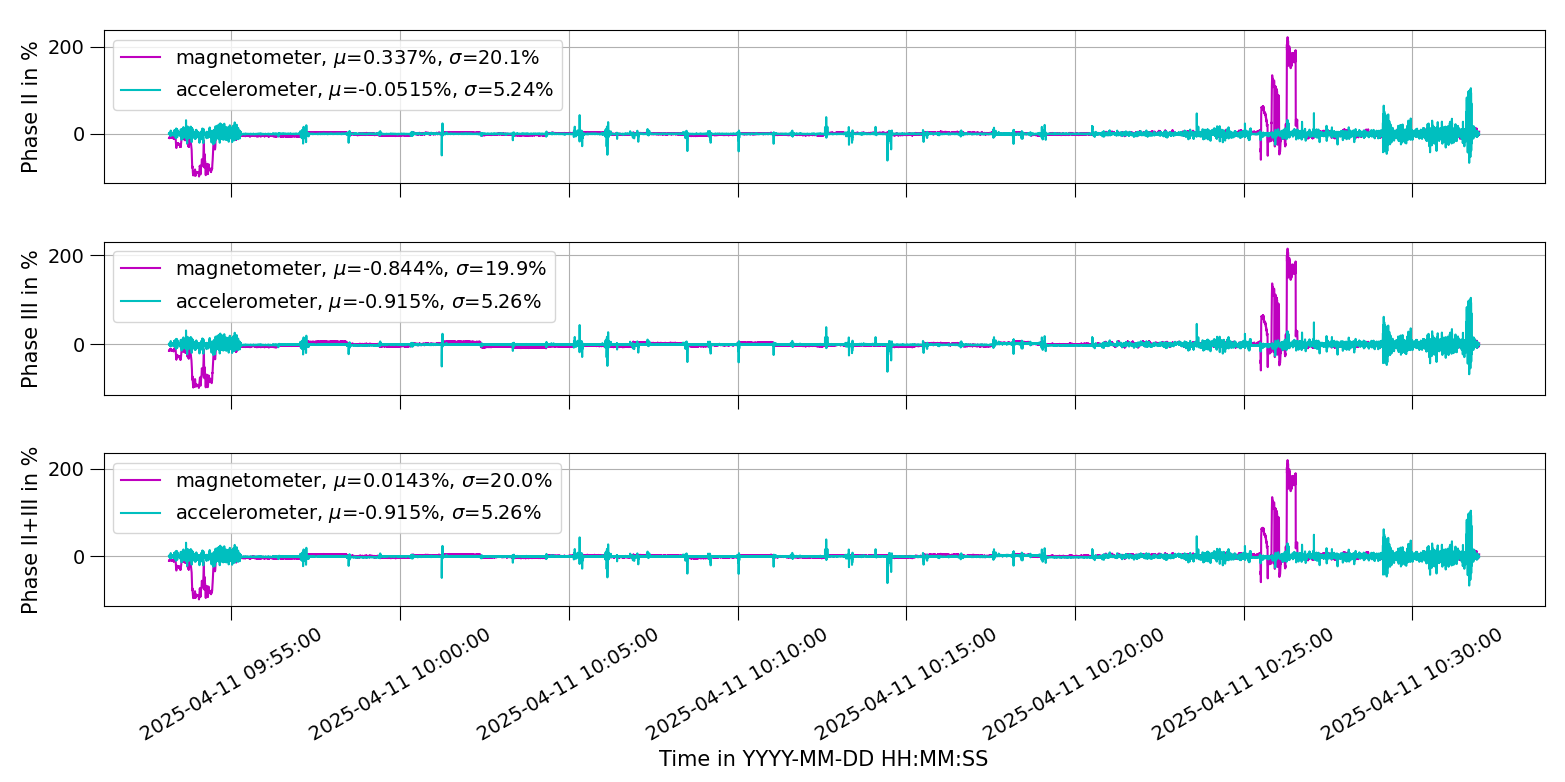
\includegraphics[width=\linewidth]{images/04_calibration/residuals_mag_acc_calibrations.png}
    \caption[Residuals of the calibrations.]{Residuals of the calibrations from top to bottom: Phase II, Phase III and Phases II+III.}
    \label{fig:res:residuals}
\end{figure}

The end of sec.~\ref{sec:app:final_coefficients} presents the calibrated curves using only the coefficients of one set. Figure~\ref{fig:res:optimal_coeff_magnitude} shows the magnitude of the data set calibrated using the optimal coefficients, as determined above. There, it can be seen that after the calibration the magnetometer shows a mostly constant magnitude. Especially during the random tumble, there is only little deviation from the constant value aside from one time moment in which the magnitude suddenly increases inexplicably.\\
However, the accelerometer paints a different picture. Even with the optimal calibration coefficients, the magnitude is not constant whenever the sensor is moved. Changing the orientation of the sensor requires a force, as per Newton's first law of motion. This force is overlaid with the gravitational force as per the superposition principle.

\begin{figure}[H]
    \centering
    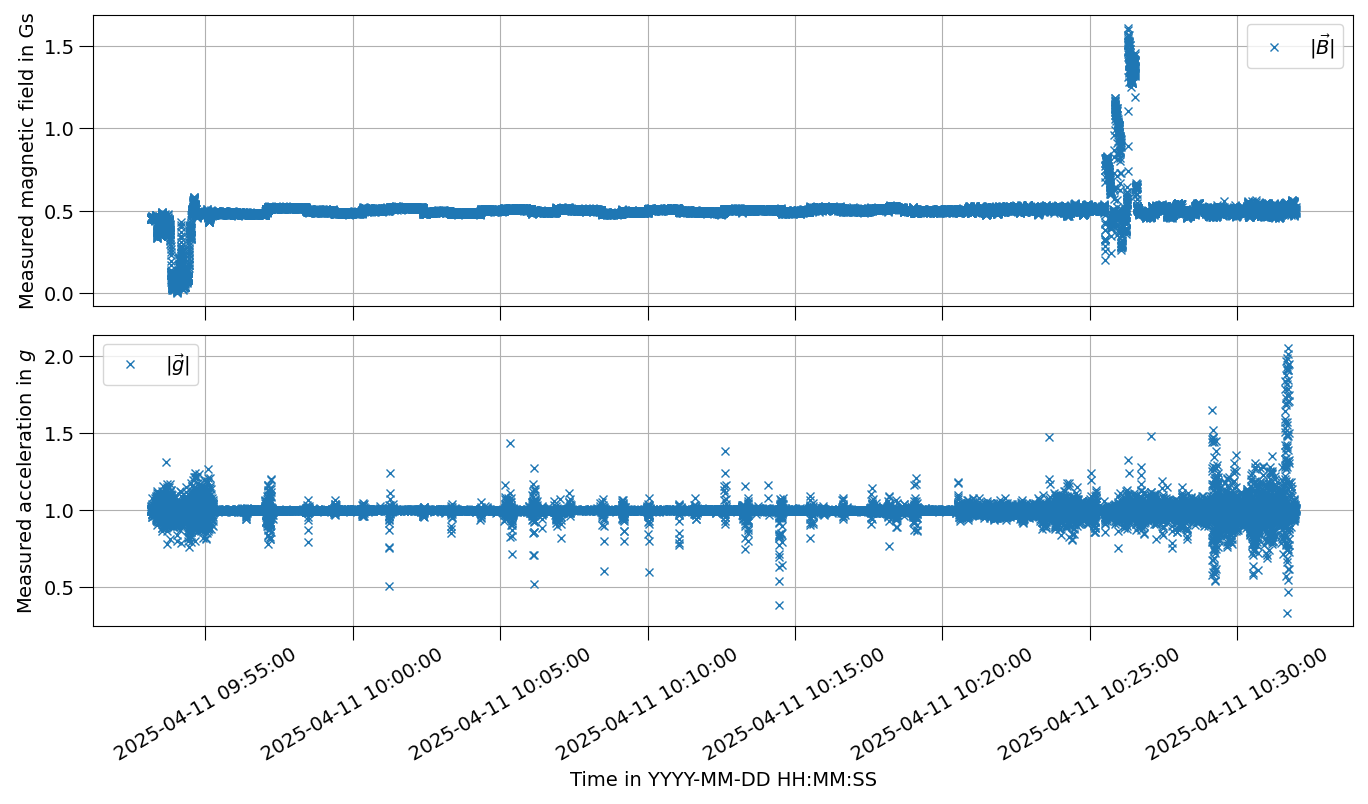
\includegraphics[width=\linewidth]{images/04_calibration/optimal_calibrated_11apr_magnitude.png}
    \caption{Magnitudes of magnetometer and accelerometer with optimal coefficients.}
    \label{fig:res:optimal_coeff_magnitude}
\end{figure}